\chapter{Controller Design}\label{ch:controldesign}
\todo[color=07controllerDesign]{Controller Design not enough text yet}
\todo[color=07controllerDesign]{Explain what PID is}
\section{Step response}
\begin{figure}[H]
    \centering
    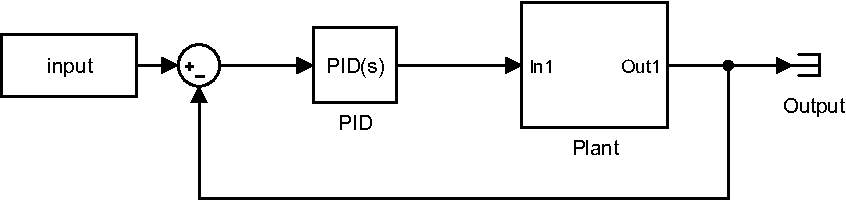
\includegraphics[width=0.75\textwidth]{figures/04ExperimentsAndLabWork/CLblock.pdf}
    \caption{A simplified block diagram to show the placement of a PID}
	\label{fig:PIDplace}
\end{figure}

For the common PID-tuning method as described by Ziegler and Nichols,
some knowledge about the system is needed.
There exist two Ziegler Nichols methods,
depending on the open-loop dynamics of the system.
Because our system has a stable response to a step input, we used the first method described in \todo[color=07controllerDesign]{page 226 ff, Feedback Control of Dynamic Systems}
Here typically a unit step input is given into the OL system as shown in figure \ref{fig:OL}.

\todo[color=07controllerDesign]{get actual values for R and L}
\begin{figure}[H]
    \centering
    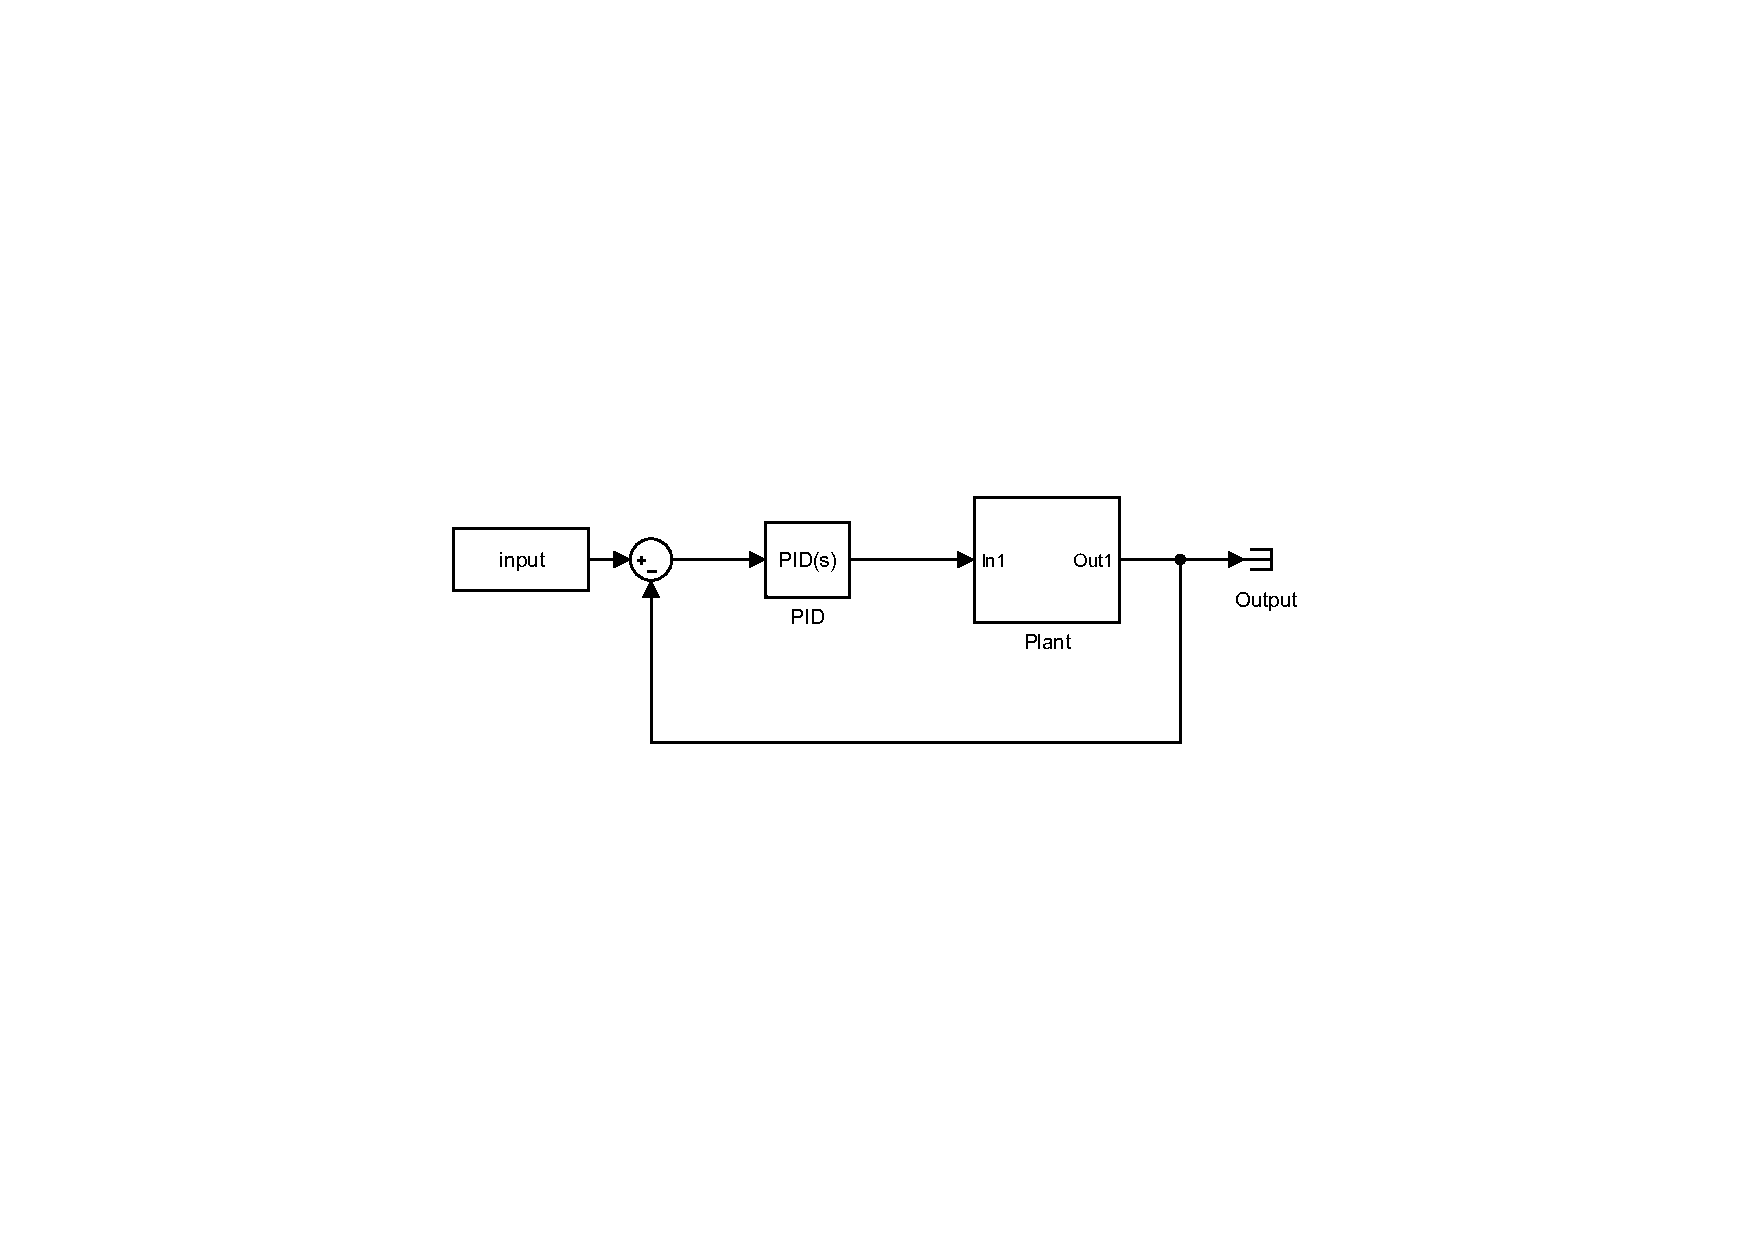
\includegraphics[width=0.75\textwidth]{figures/04ExperimentsAndLabWork/OLblock.pdf}
    \caption{OL block diagram of the system}
\label{fig:OL}
\end{figure}

Because we are scaling the $\omega$ down by a factor of 10, so we can directly read the percentage,
we had to scale the aforementioned unit step up by a factor of 10,
in order to get usable results.
While encountering this problem, we also noticed, that the pumps don't spin below an $\omega$ of 9\%.
When using the corrected step input, we got the measurements shown in figure X \ref{fig:stepin}.

Our analysis of figure \ref{fig:stepin} gives us the following values:
\\
\begin{tabular}{r c l l}
	$A$ 	& $=$ & $2.2177$ 	& \footnotesize{\textit{final value}}\\
	$R$ 	& $=$ & $1.7833$ 	& \footnotesize{\textit{slope}}\\
	$t_d=L$	& $=$ & $0.75$ 		& \footnotesize{\textit{lag}}\\
	$\tau$ 	& $=$ & $1.2436$ 	& \footnotesize{\textit{time constant}}
\end{tabular}
\\
Ziegler-Nichols is tuning a PID controller $D_c(s)$ with the formula\\
$D_c(s)=k_P(1+ \frac{1}{T_Is}+T_Ds)$,
where $k_P$, $T_I$ and $T_D$ are scalar gains,
tuned according to the characteristics obtained from figure \ref{fig:stepin}.

\begin{tabular}{r c l l}
	$k_p$ & $=$ & $\nicefrac{1.2}{RL}$	& \footnotesize{\textit{proportional gain}}\\
	$T_I$ & $=$ & $2L$					& \footnotesize{\textit{integral gain}}\\
	$T_D$ & $=$ & $0.5L$ 				& \footnotesize{\textit{derivative gain}}\\
\end{tabular}


\begin{figure}[H]
    \centering
    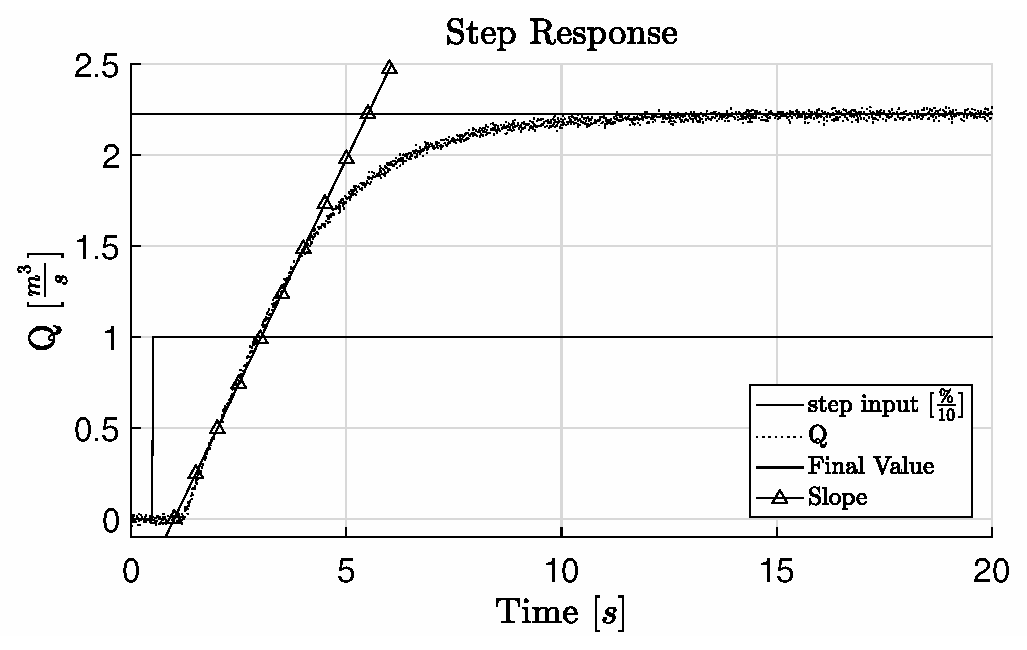
\includegraphics[width=\textwidth]{figures/04ExperimentsAndLabWork/StepResponseLabeled.eps}
    \caption{response to a step input with value 10}
	\label{fig:stepin}
\end{figure}
\todo[color=07controllerDesign]{can we make the axis look like they are made by LaTeX as well?}
\\ \\ \\ \\
\todo[color=07controllerDesign]{structure}